\documentclass[paper=a4, fontsize=10pt]{scrartcl}

\linespread{1.05}

\usepackage{physics-math}
\usepackage{pgfplotstable, booktabs}


\setlength\parindent{0pt} 

\title{Lab Report - Magnetisation}
\subtitle{Advanced lab course in
  physics for Master students - experiment: magnetisation studies}
\author{Alexander Kreuzer, Simon Fromme}
\date{\normalsize\today}


\begin{document}
\maketitle

\section{Calibration of the SQUID}

Since the SQUID outputs only a voltage signal and no direct
information about the magnetic field $B$, we need to perform some sort
of calibration first in order to obtain the correct relationship of
$B$ to the output voltage of the SQUID $\si{U}_{SQUID}$.

\subsection{Calibration by means of a solenoid}

Using Biot-Savarts law we can estimate the relationship between the
electric current in the solenoid $I_{\mathrm{Sol}}$ and the magnetic
field at the SQUID $B_{\mathrm{SQUID}}$ to be
\begin{align*}
  B_{\mathrm{SQUID}}(I_{\mathrm{Sol}}) = \mu_0 \dfrac{R^2}{2|x|^3} I_{\mathrm{Sol}}.
\end{align*}
With the solenoid radius $R=\SI{0.35}{\cm}$ and the distance ``solenoid
- SQUID'' $x=\SI{1.4}{\cm}$ we thus obtain
\begin{align}
  B(I_{\mathrm{Sol}}) = \SI{2.805e-5}{G\per\m\A} \cdot I_{\mathrm{Sol}}. \label{eq:magnetic-field-squid}
\end{align}
\par

In the experiment we now varied the electric current in the solenoid
and measured the corresponding output voltage of the SQUID to obtain a
relationship between both quantities.

Since the reading of the voltmeter was quite fluctiating during the
course of a single measurement, each measurement of
$S_{\mathrm{SQUID}}$ was performed over an interval of ca.
$\SI{5}{\s}$ and both minimum and maximum voltage during that time was
noted. The results are listed in table \ref{tab:calibration_solenoid}.

\pgfplotstableread{data/1_a_soneloid.dat}\datatable
\pgfplotstabletranspose[string type]\mytablenew{\datatable}

\begin{table}
  \centering
\pgfplotstabletypeset[
    every head row/.style={ 
        output empty row,
        before row={%
            \toprule
        }
      },
    every row no 0/.style={
      after row=\midrule
    },
    every last row/.style={
      after row=\bottomrule
    },
    create on use/newcol/.style={
      create col/set list={$I_{\mathrm{Sol}}$ in $\si{mA}$,
                           $U_{\mathrm{min}}$ in $\si{mV}$,
                           $U_{\mathrm{max}}$ in $\si{mV}$}
    },
    columns/newcol/.style={string type},
    %TODO: Make this independent of colum number
    columns={newcol,0,1,2,3,4,5,6,7,8,9,10}
    ]{\mytablenew}%{\datatable}
    \caption{SQUID voltage $U$ dependence on solenoid current
      $I_{\mathrm{Sol}}$ }
    \label{tab:calibration_solenoid}
\end{table}

Using a simple linear regression model we then obtain the relationship
% Maybe even that can be made dynamic?!
\[ U_{\mathrm{SQUID}}(I_{\mathrm{Sol}}) = \SI{-0.045}{mV\per mA}\cdot
  I_{\mathrm{Sol}} + \SI{38.068}{mV} \]
and thus with (\ref{eq:magnetic-field-squid})
\[ B(U_{\mathrm{SQUID})}) = -\SI{6.159e-4}{G\per mV} \cdot
  U_{\mathrm{SQUID}} + \SI{2.345e-2}{G} \]

\begin{figure}
  \centering
  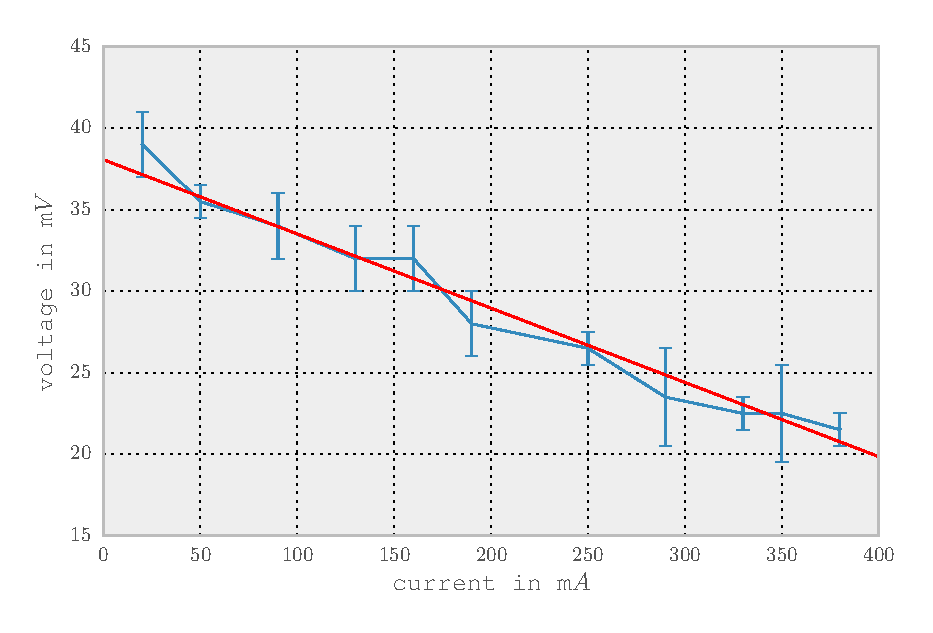
\includegraphics{plots/1_a_solenoid_calibration}
  \caption{Linear regression to determine a relation between SQUID
    voltage and solenoid current. Error bars indicate the threshold
    between the maximum and minimum measured value}
\end{figure}

\subsection{Calibration by means of a nickel sample}

In the second calibration method we (partially) magnetize a nickel
sample by placing it in the (approximately) homogeneous magnetic field
of a solenoid. Since the Curie temperature of nickel is known to be
well above room temperature\footnote{$T_{\mathrm{C}} = \SI{633}{K}$},
both the initial magnetisation and SQUID measurements can be performed
without cooling without altering the ferromagnetic properties of the
sample.

The solenoid current $I_{\mathrm{Sol}} = \SI{1}{A}$ used corresponds
to a magnetic field of $B_{\mathrm{Sol}} = \SI{1000}{G}$\footnote{In
  the auxiliary material the relationship
  $B(I_{\mathrm{Sol}}) [\si{G}] = 0.9846 \cdot I_{\mathrm{Sol}}
  [\si{mA}] + 2,059$ was given. According to the supervisor of the
  experiment this accuracy does not reflect the actual experimental
  setup.}.

% citation needed for Curie temperature of nickel

With the values for the mass density\footnote{We did use the published
  value of $\rho_{\mathrm{pub}} = \SI{8912}{\kg\per\cubic m}$, rather
  than calculating it ourselves from
  $\rho_{\mathrm{exp}} = m/V = \SI{2.2e-5}{\kg} ~/~ \SI{2.5e-9}{\cubic
    m} = \SI{8080}{\kg\per\cubic m}$ as suggested in the experiment
  description.} $\rho = \SI{8912}{\kg\per\cubic m}$ of the sample and
the specific saturation magnetisation of nickel
$\sigma_{\mathrm{Sat}} = \SI{55.09}{A\square\m\per\kg}$ given in the
auxiliary material we obtain
\[ M_{\mathrm{Sat}} = \sigma_{\mathrm{Sat}} \cdot \rho =
  \SI{4.91e5}{A\per\m}. \]

The necessary magnetic field for saturation is then
\begin{align*}
  B_{\mathrm{Sat}} = \mu_0 \cdot M_{\mathrm{Sat}} = \SI{6170}{G}.
\end{align*}
Since $B_{\mathrm{Sat}} > B_{\mathrm{Solenoid}}$, we cannot fully
magnetize the sample and will assume a linear relationship between
$B_{\mathrm{Solenoid}}$ and the resulting magnetisation $M$ to account
for this fact. For the actual magnetisation we obtain
\[ B = \dfrac{\mu_0}{2\pi} \dfrac{\mu}{x^3} = \dfrac{\mu_0}{\pi}
  \dfrac{m\sigma_S}{x^3}\dfrac{B_{\mathrm{Solenoid}}}{B_{\mathrm{Sat}}}
  = \SI{1.31e-5}{T} = \SI{0.131}{G}, \] where $\mu$ is the total
magnetic moment and $m = \SI{0.0202}{g}$ is the mass of the sample.

Taking three different measurements (only copper base/perpendicular
nickel orientation/parallel nickel orientation) with six values each,
we obtain the values and respective averages listed in table
\ref{table:nickel-squid}.

\begin{table}[h]
  \centering
\begin{tabular}{l|c|c|c|c|c|c|c}
  orientation & \multicolumn{6}{c|}{$U_{\mathrm{SQUID}}$ in $\si{V}$} & $\bar{U}_{\mathrm{SQUID}}$ in $\si{V}$\\
  \toprule
only copper base & 0.451 & 0.455 & 0.457 & 0.449 & 0.459 & 0.467 & 0.456\\ 
parallel & 0.634 & 0.612 & 0.632 & 0.615 & 0.606 & 0.619 & 0.620\\ 
perpendicular & 0.626 & 0.624 & 0.622 & 0.620 & 0.626 & 0.623 & 0.624\\
  \bottomrule
\end{tabular}
\caption{SQUID-calibration with a nickel sample}
\label{table:nickel-squid}
\end{table}
Since Copper is not ferromagnetic it does not have a permanent
magnetisation and if further assume that the influences of the
magnetic field induced by the sample on the copper base can be
neglected we can estimate $M(U) = M(U-U_{\mathrm{base}})$:

\begin{itemize}
\item perpendicular orientation: \\
  \begin{align*}
    M_{\mathrm{perp}}(U) = \alpha_{\mathrm{perp}} \l( {U - U_{\mathrm{base}}} \r) &\qquad \mathrm{with}~~\alpha_{\mathrm{perp}} = \SI{4.76e5}{A\per m \per V} \\
    B_{\mathrm{perp}}(U) = \beta_{\mathrm{perp}} \l( {U - U_{\mathrm{base}}} \r) &\qquad \mathrm{with}~~\beta_{\mathrm{perp}} = \SI{0.783}{G \per V}
  \end{align*}
\item parallel orientation:
  \begin{align*}
    M_{\mathrm{parallel}}(U) = \alpha_{\mathrm{parallel}} \l( {U - U_{\mathrm{base}}} \r) &\qquad \mathrm{with}~~\alpha_{\mathrm{parallel}} = \SI{4.87e5}{A\per m \per V} \\
    B_{\mathrm{parallel}}(U) = \beta_{\mathrm{parallel}} \l( {U - U_{\mathrm{base}}} \r) &\qquad \mathrm{with}~~\beta_{\mathrm{parallel}} = \SI{0.802}{G \per V}
  \end{align*}
\end{itemize}

Where we will use $\alpha_{\mathrm{perp}}$
($\alpha_{\mathrm{parallel}}$) for perpendicular (parallel) mounting
of the sample.

In the following we will use the calibration factors obtained from the
second method.


\section{measurements of magnetisation}

\subsection{terbium sample (perpendicular mounting)}
Mounting the cooled down terbium sample perpendicular the temperature
dependence of its magnetisation was measured for the three cases
\begin{itemize}
\item cooling down \emph{with no} applied magnetic field, no magnetic field
  applied afterwards
\item cooling down \emph{with no} applied magnetic field, subsequent
  magnetisation at low temperature with $B = \SI{150}{G}$
\item cooling down \emph{with} applied magnetic field ($B = \SI{150}{G}$)  
\end{itemize}
Starting from a temperature of about $\SI{90}{K}$ the sample was
heated up with hot air until it reached about $\SI{250}{K}$. Using the
calibration factors obtained the resulting dependence of
$B_{SQUID}(T)$ is shown in figure \ref{fig:terbium_perpendicular}.

\begin{figure}
  \centering
  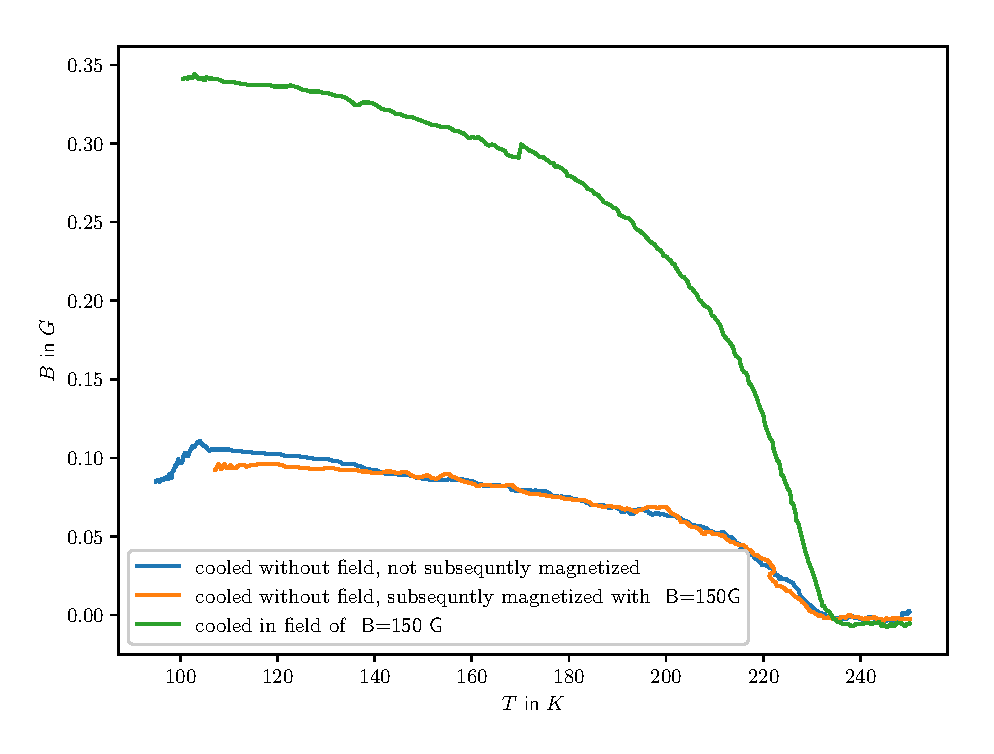
\includegraphics{plots/2_a_perpendicular}
  \caption{$B_{\mathrm{SQUID}}$ measurements for perpendicular
    mounting of terbium. Calibration was done according to 1.b,
    additionally an offset on $B = -0.11/ -0.07/ \SI{0.07}{G}$ was
    added to ensure $B \rightarrow 0$ for
    $T \rightarrow \SI{270}{K}$.}
  \label{fig:terbium_perpendicular}
\end{figure}

It can be seen, that only terbium cooled down in the magnetic field of
$\SI{150}{G}$ shows a significant magnetisation. Starting from an
initial magnetisation, the magnetisation vanishes approximately
according to $B(T) \propto \dfrac{1}{T-T_C}$ until it reaches a critical
temperature $T_{C}$ where it reaches 0. For $T>T_C$ the sample is
paramagnetic.

The samples not cooled down in a magnetic field (regardless of whether
a field was applied afterwards or not) show almost no initial
magnetisation\footnote{The still existing initial magnetisation for
  the two samples may be explained by electromagnetic noise fields
  still present during the cool down process.}




\subsection{terbium sample (parallel mounting)}

Mounting the terbium sample parallely we determined the $B-T$
relationship for three different initial magnetisations (cooling down
in a field of $B \in \{ \SI{50}{G}, \SI{100}{G}, \SI{150}{G}\}$). We
obtain the curves depicted in figure \ref{fig:terbium_parallel}.


\begin{figure}
  \centering
  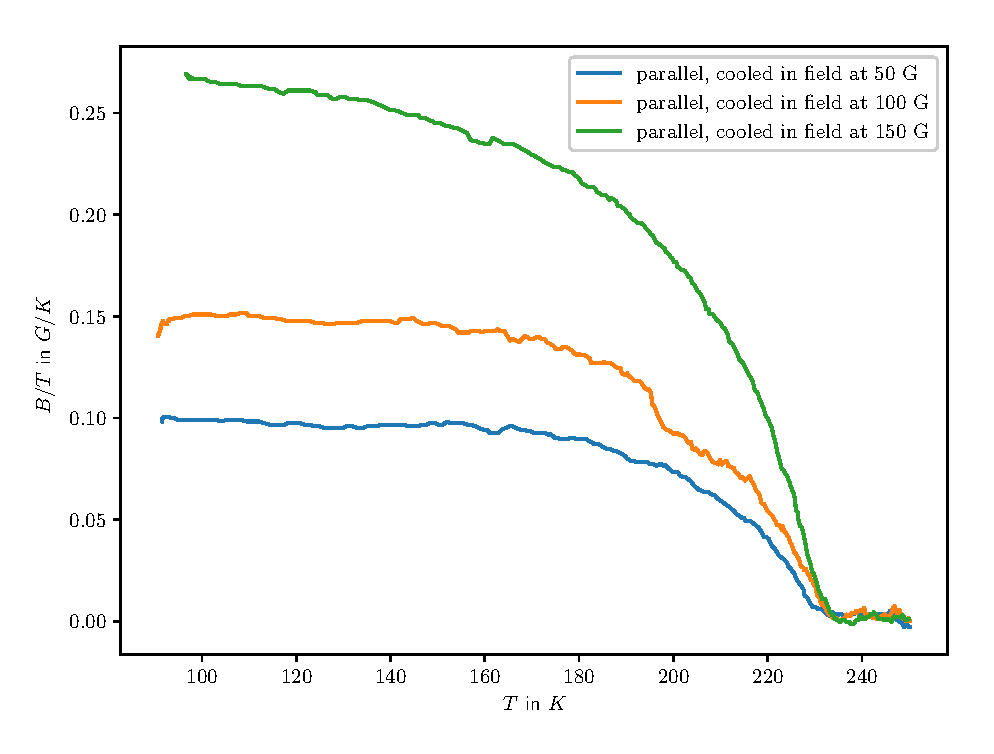
\includegraphics{plots/2_b_parallel}
  \caption{Temperature dependence ot terbium (parallel orientation)
    with different initial magnetisations. Calibration was done
    according to 1.b, additionally an offset on
    $B = -0.01/ -0.04/ \SI{-0.01}{G}$ was added to ensure
    $B \rightarrow 0$ for $T \rightarrow \SI{270}{K}$.}
  \label{fig:terbium_parallel}
\end{figure}

It can be seen, that the initial magnetisation scales linearly with
the magnetic field in the solenoid since no saturation was reached. Up
until reaching the phase transition to the paramagnetic state the
magnetisation vanished according to the Curie law
$\propto \dfrac{1}{T-T_C}$. When reaching the paramagnetic state the
magnetisation reaches 0 for all initial magnetisations. A helimagnetic
state (as mentioned in the preparation material) could not be seen.


\subsubsection{Curie temperature}


Calculating the derivative
$\dfrac{\textrm{d}}{\textrm{d} T}B_{\mathrm{SQUID}}(T)$ from a moving
average (calculated over 30 datapoints) of both $T$ and
$U_{\mathrm{SQUID}}$ we find it has minimums for the following
temperatures. The respective curves are shown in figure
\ref{fig:terbium_derivation}.

\begin{table}[h]
  \centering
\begin{tabular}{l|c}
  sample & $T_{\mathrm{C}}$ in $\si{K}$\\
  \toprule
parallel, cooled down in field at $\SI{50}{G}$ & 229.53 \\
parallel, cooled down in field at $\SI{100}{G}$ & 231.91 \\
parallel, cooled down in field at $\SI{150}{G}$ & 229.40 \\
 perpendicular, cooled down in field at $\SI{150}{G}$ & 232.17 \\
  \bottomrule
\end{tabular}
\caption{estimates of $T_{\mathrm{C}}$ for a differently magnetized
  terbium sample}
\label{table:nickel-squid}
\end{table}
Hence, we can estimate the Curie temperature $T_C$ (temperature of the
phase transition from ferromagnetic to paramagnetic state) by
averaging these values and arrive at an estimate of
\begin{align*}
   T_C^{\mathrm{avg}} = \SI{230.75}{K}. 
\end{align*}

The minima vary within a range of approximately
$\Delta T = \SI{3}{K}$, which partially might be explained by the fact
that the minimum of the derivation
$\dfrac{\textrm{d}}{\textrm{d} T}B_{\mathrm{SQUID}}(T)$ is not exactly
the point where $B_{\mathrm{SQUID}}$ reaches 0.

\begin{figure}
  \centering
  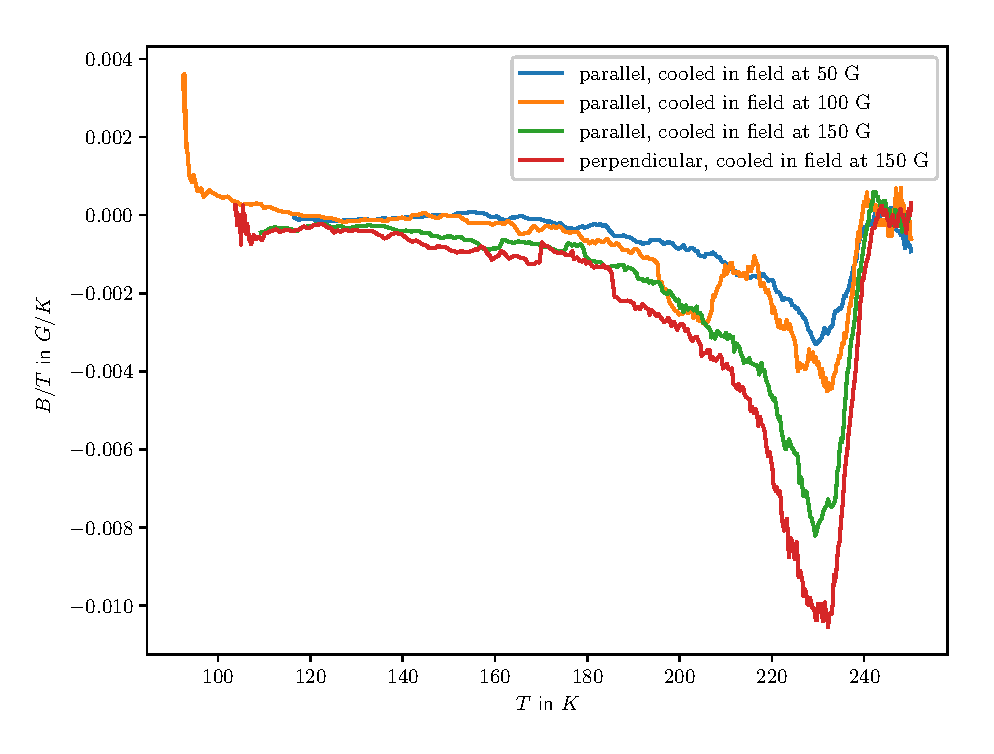
\includegraphics{plots/2_derivation}
  \caption{Derivation of temperature dependence ot terbium (parallel
    orientation) with different initial magnetisations. The derivation
    was calculated over a moving average of a 30-point window for both
    temperature and magnetic field.}
  \label{fig:terbium_derivation}
\end{figure}

\subsection{gadolinium sample}

In the last part a gandolinium sample was initially magnetized with
$B = \SI{1000}{G}$ and all measurements carried out just as in the
terbium case. The magnetisation falls down at
$T_{C} \approx \SI{290}{K}$ when reaching the paramagnetic state.

The behaviour for $T$ between ca. $\SI{225}{K}$ and $\SI{290}{K}$ is
quite interesting. The rise of $B$ can be explained by the turning of
the magnetisation axis with respect to the measurement axis of the
SQUID. The former turns towards the latter for $T > \SI{200}{K}$.


\begin{figure}
  \centering
  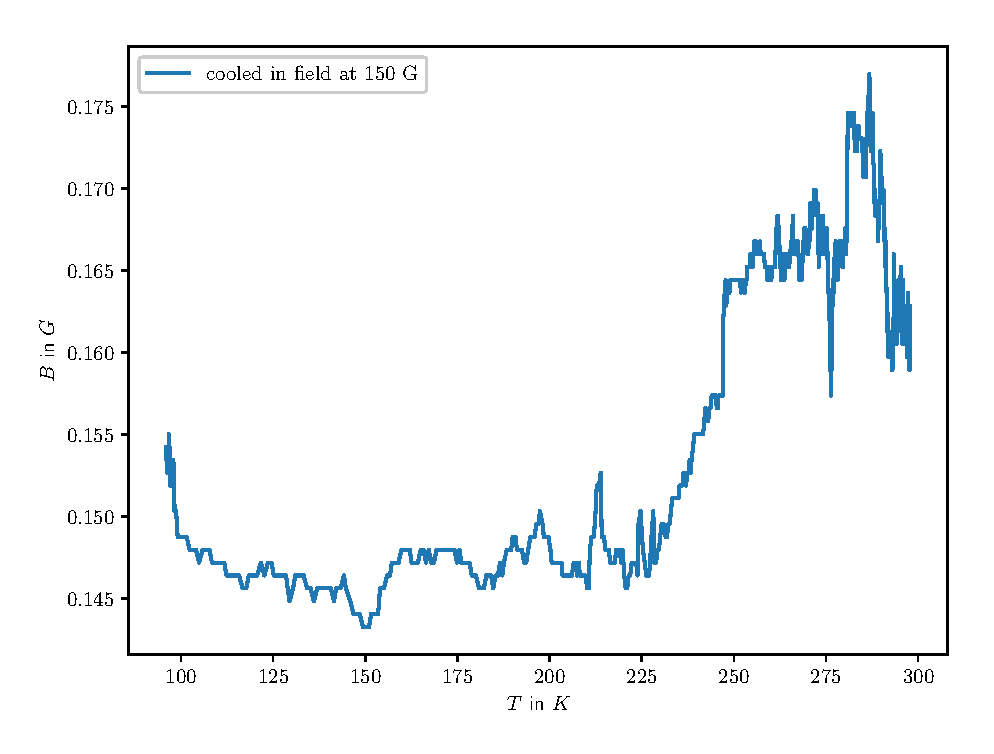
\includegraphics{plots/3_gandolinium}
  \caption{$B-T$ relationship for gandolinium}
  \label{fig:terbium_derivation}
\end{figure}


\end{document}
